%%%%%%%%%%%%%%%%%%%%%%%%%%%%%%%%%%%%%%%
% a0poster Landscape Poster
% LaTeX Template
% Version 1.0 (22/06/13)
%
% The a0poster class was created by:
% Gerlinde Kettl and Matthias Weiser (tex@kettl.de)
% 
% This template has been downloaded from:
% http://www.LaTeXTemplates.com
%
% License:
% CC BY-NC-SA 3.0 (http://creativecommons.org/licenses/by-nc-sa/3.0/)
%
%%%%%%%%%%%%%%%%%%%%%%%%%%%%%%%%%%%%%%%%%

%----------------------------------------------------------------------------------------
%	PACKAGES AND OTHER DOCUMENT CONFIGURATIONS
%----------------------------------------------------------------------------------------

% aspb is 3'7'' x 3'6''
\documentclass[aspb,landscape]{a0poster}

\usepackage{fontspec}
\usepackage[svgnames]{xcolor} % enable specifying colors by their 'svgnames', for a full list of all colors available see here: http://www.latextemplates.com/svgnames-colors

% Carnegie uses Roboto Slab (serif) and Lato (sans serif)
\setmainfont[Ligatures=TeX]{Lato}

% Carnegie colors
\definecolor{CarnegiePriBlue}{cmyk}{1.00,0.85,0.15,0.25}  % main primary blue
\definecolor{CarnegieSecBlue1}{cmyk}{0.68,0.48,0.00,0.00} % first secondary blue
\definecolor{CarnegieSecBlue2}{cmyk}{0.85,0.69,0.04,0.00} % second secondary blue

\definecolor{CarnegiePriTurq}{cmyk}{0.60,0.10,0.15,0.00}  % main primary turquoise

\definecolor{CarnegiePriGreen}{cmyk}{0.46,0.00,0.90,0.00} % main primary green

\definecolor{CarnegiePriBrown}{cmyk}{0.25,0.40,0.65,0.00} % main primary brown

% multiple columns
\usepackage{multicol} % This is so we can have multiple columns of text side-by-side
\columnsep=100pt      % This is the amount of white space between the columns in the poster
\columnseprule=3pt    % This is the thickness of the black line between the columns in the poster
\def\columnseprulecolor{\color{lightgray}}

% other needed packages
\usepackage{amsfonts, amsmath, amsthm, amssymb} % For math fonts, symbols and environments
\usepackage{wrapfig}  % Allows wrapping text around tables and figures
\usepackage{graphicx} % Required for including images
\usepackage{booktabs} % Top and bottom rules for table

% tweak figure and table captions
\usepackage[font=small,labelfont={bf,color=CarnegiePriBlue},textfont={color=CarnegiePriBlue},margin=0pt,skip=18pt]{caption}

% natbib drops numbers and we'll shrink text size; drop labels
\usepackage{natbib}
\def\bibfont{\footnotesize}
\makeatletter
\renewcommand\@biblabel[1]{}
\makeatother

% tweak list spacing
\usepackage{enumitem}
\setlist[itemize]{topsep=10pt,itemsep=8pt,itemindent=48pt}
\setlist[enumerate]{topsep=10pt,itemsep=8pt,itemindent=0pt}


% tweak paragraphs
\setlength{\parindent}{0pt}
\setlength{\parskip}{12pt}

% tweak title spacing and colors
% \titlespacing{command}{left spacing}{before spacing}{after spacing}[right]
% spacing: how to read {12pt plus 4pt minus 2pt}
%          12pt is what we would like the spacing to be
%          plus 4pt means that TeX can stretch it by at most 4pt
%          minus 2pt means that TeX can shrink it by at most 2pt
\usepackage{titlesec}

\titlespacing{\section}{0pt}{24pt}{12pt}
\titlespacing{\subsection}{0pt}{12pt}{12pt}
\titlespacing{\subsubsection}{0pt}{12pt}{12pt}

\titleformat{\section}{\color{CarnegiePriBlue}\Large\bfseries}{\color{CarnegiePriBlue}\thesection}{1em}{}
\titleformat{\subsection}{\color{CarnegiePriBrown}\large\bfseries}{\color{CarnegiePriBrown}\thesubsection}{1em}{}

% tweak equation whitespace
%% \abovedisplayskip=12pt plus 3pt minus 9pt
%% \abovedisplayshortskip=0pt plus 3pt
%% \belowdisplayskip=12pt plus 3pt minus 9pt
%% \belowdisplayshortskip=7pt plus 3pt minus 4pt

% width of figures for consistency
\newlength{\figwidth}
\setlength{\figwidth}{240mm}

% space above figures
\newlength{\figtopspace}
\setlength{\figtopspace}{10pt}

\graphicspath{{figures/}} % Location of the graphics files

%% % DEBUG: overlay a grid to view spacing
%% \usepackage[grid,gridcolor=red!20,subgridcolor=green!20,gridunit=in]{eso-pic}

\begin{document}

%----------------------------------------------------------------------------------------
%	POSTER HEADER 
%----------------------------------------------------------------------------------------

% The header is divided into three boxes:
% The first is 55% wide and houses the title, subtitle, names and university/organization
% The second is 25% wide and houses contact information
% The third is 19% wide and houses a logo for your university/organization or a photo of you
% The widths of these boxes can be easily edited to accommodate your content as you see fit
% Note: no line breaks between minipage environments!

\textbf{\color{CarnegiePriBlue} \VeryHuge Model-Based Quantification of Induced Gene Expression Time Courses}    % Title

\begin{minipage}[m]{0.08\linewidth}
  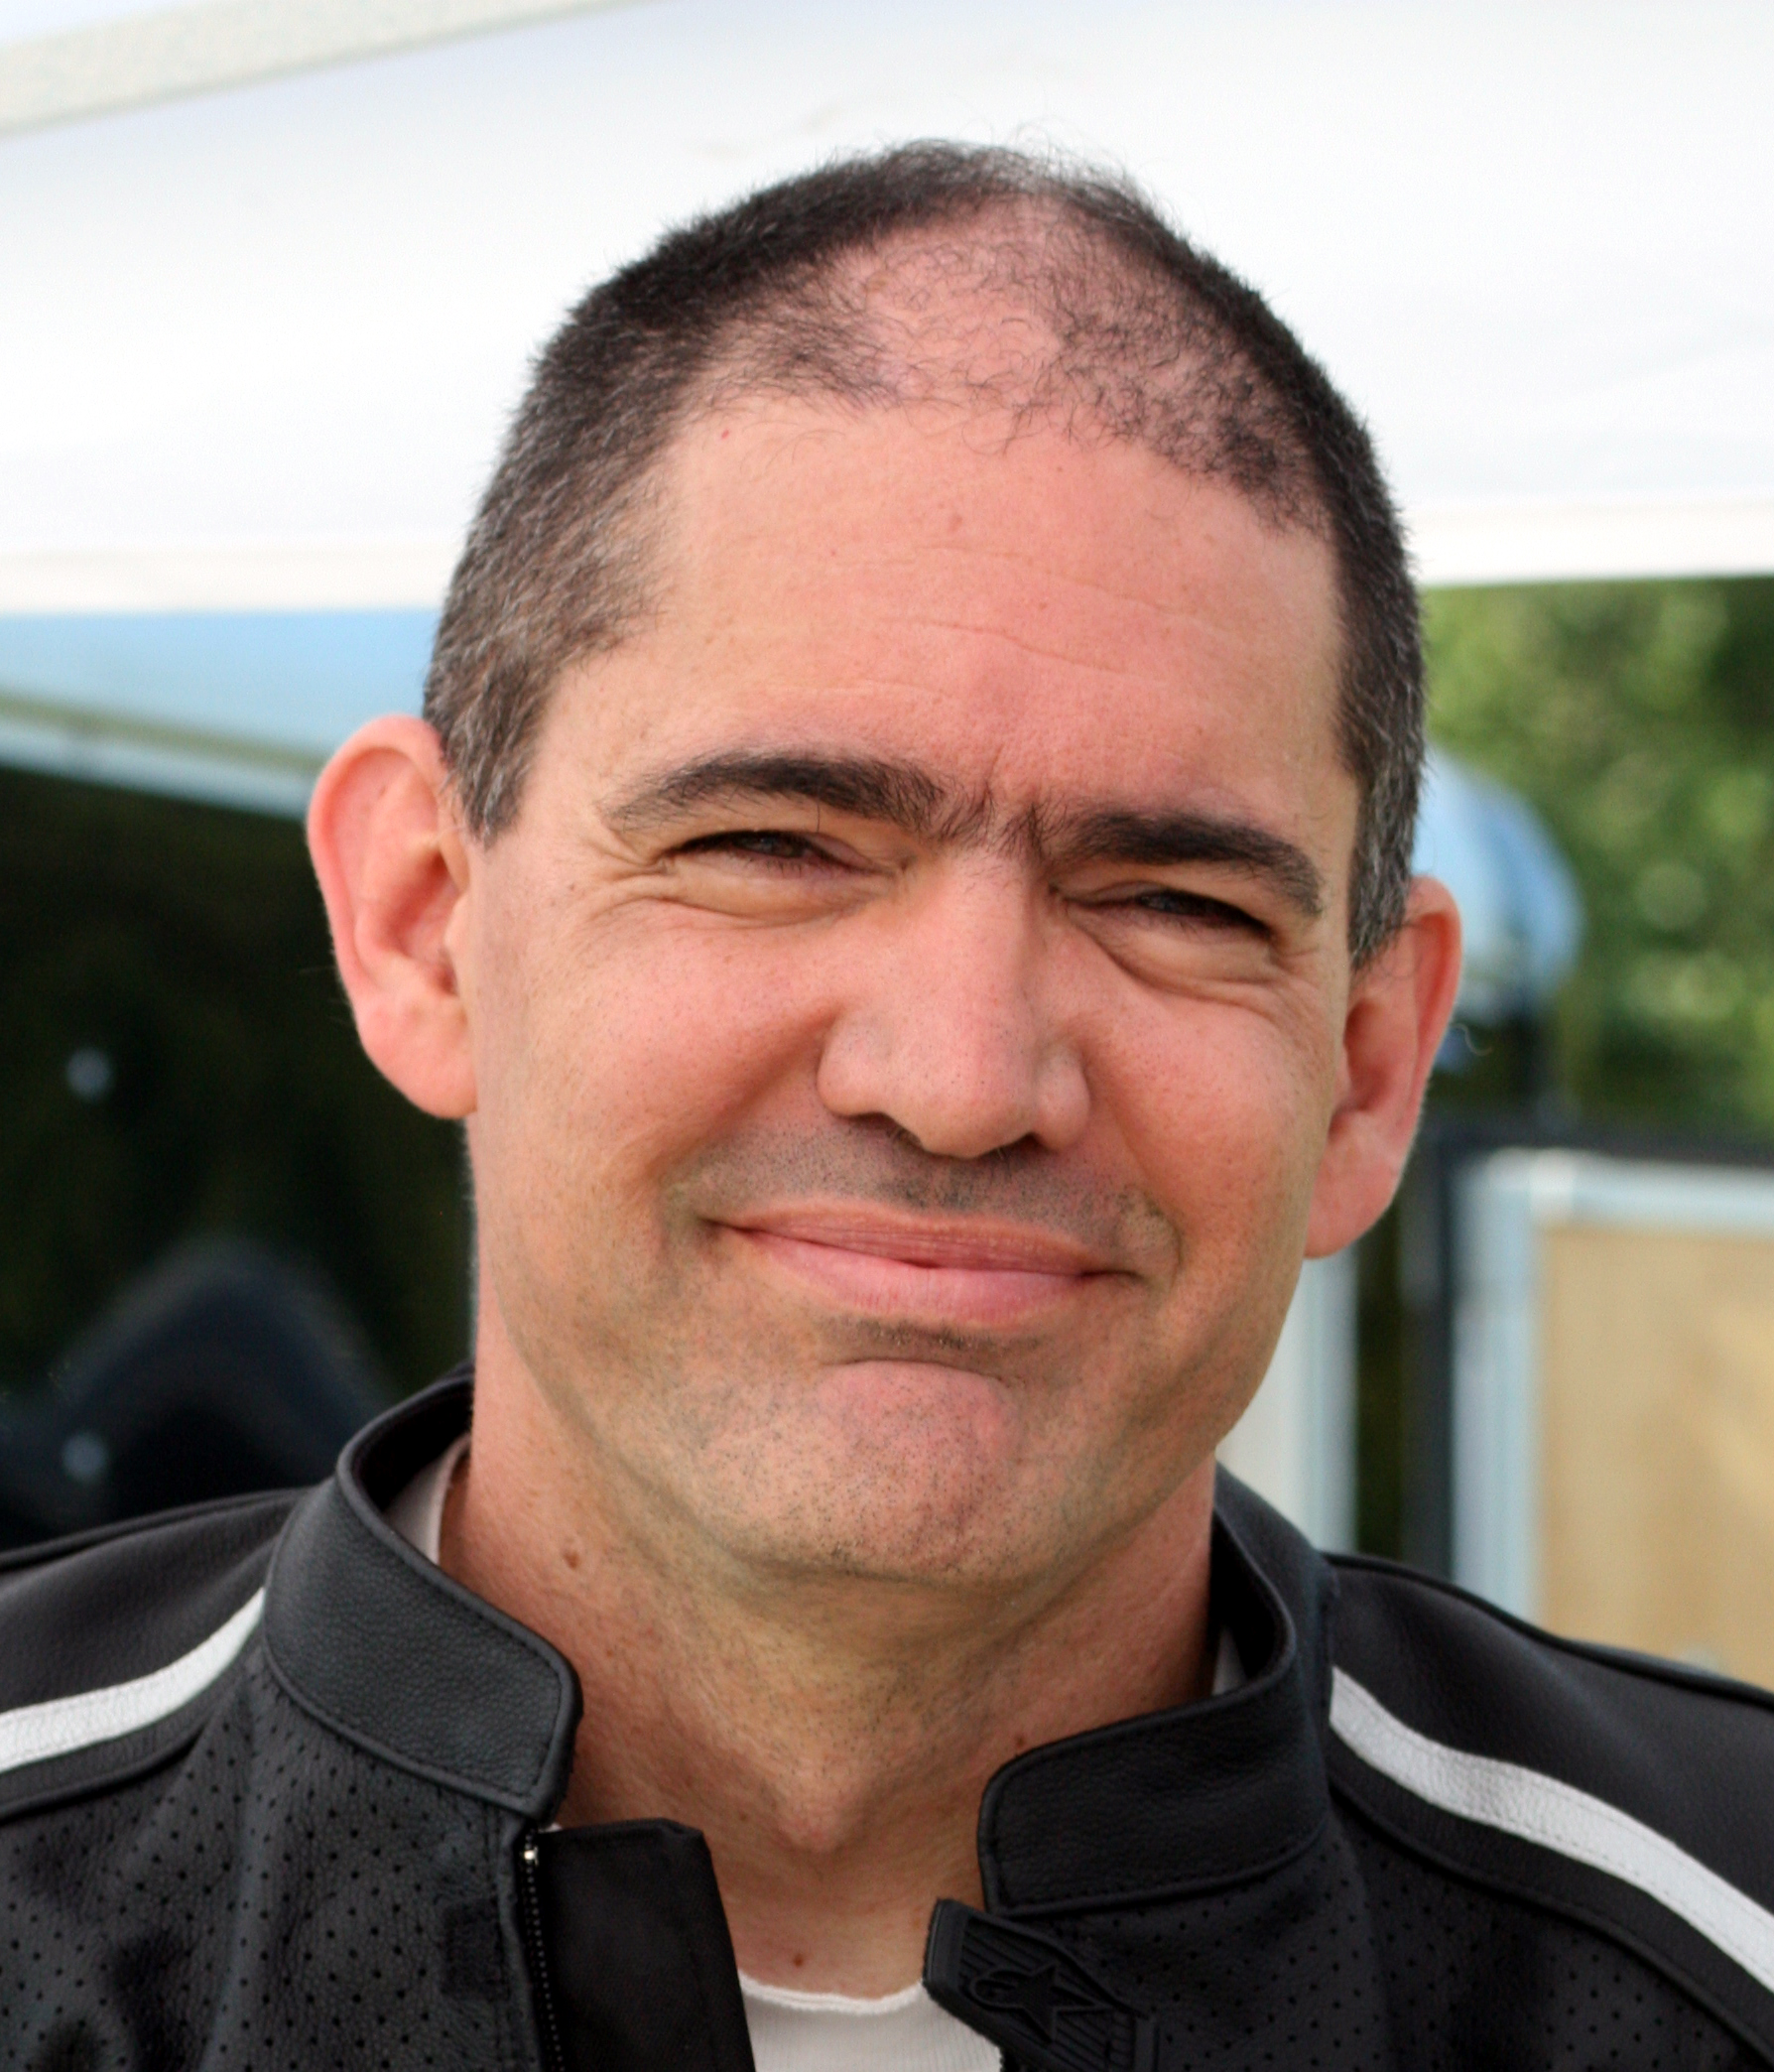
\includegraphics[height=50mm]{sam-bfr-smiling-crop.jpg} % author photo
\end{minipage}
\begin{minipage}[m]{0.40\linewidth}                      % Author(s)
  \color{Black}
  \Huge \textbf{Sam Hokin \& M. Kathryn Barton} \\
  \Large shokin@carnegiescience.edu
\end{minipage}
\hfill
\begin{minipage}[m]{0.40\linewidth}                      % Author(s)
  \hfill
  
\includegraphics[height=50mm]{CS_plantbio_logo_horz.eps} % Carnegie DPB logo
\end{minipage}

\vspace{5mm} % A bit of extra whitespace between the header and poster content
\color{CarnegiePriBlue}
\hrulefill

\color{Black}

%% \color{DarkSlateGray}\Large \textbf{Contact Information:}\\
%% Department Name\\ % Address
%% University Name\\
%% 123 Broadway, State, Country\\\\
%% Phone: +1 (000) 111 1111\\ % Phone number
%% Email: \texttt{john@LaTeXTemplates.com}\\ % Email address


%----------------------------------------------------------------------------------------

\begin{multicols}{4} % This is how many columns your poster will be broken into, a poster with many figures may benefit from less columns whereas a text-heavy poster benefits from more

  \color{Black} % default color

  %----------------------------------------------------------------------------------------
  %	ABSTRACT
  %----------------------------------------------------------------------------------------

  %% \begin{abstract}
  %% \end{abstract}

  %----------------------------------------------------------------------------------------
  %	INTRODUCTION
  %----------------------------------------------------------------------------------------

  {
    \titlespacing{\section}{0pt}{0pt}{0pt} % suppress skip on very first section
    \section*{INTRODUCTION}
  }

  \textbf{We model gene expression time courses following induction of a glucocorticoid receptor-bound transcription factor into the nucleus due to exposure to dexamethasone in Arabidopsis thaliana.}
  
  In contrast to measurement of induced expression at a single time, resulting in a single fold-change value typically long after the induction event,
  we model the dynamics of TF import into the nucleus followed by the transcriptional dynamics of its direct and indirect targets.
  
  \textbf{The model quantifies an observed time course with two rate coefficients}:
  \begin{enumerate}
  \item $\hat{\eta}_p$ = the normalized initial rate of rise (+) or fall (-) of target mRNA levels
  \item $\gamma_p$ = the mRNA loss rate
  \end{enumerate}
  \textbf{These two processes compete to determine the final transcript fold change:} a highly-induced transcript may saturate at a low fold change if it also decays quickly,
  while weakly-induced transcripts may rise to a high level if they have very low loss.
  
  \textbf{In addition, some targets exhibit ``turn-off'', or auto-regulation}. These time courses require a turn-off time, $t_{off}$, after which the mRNA level decays exponentially at $\gamma_p$.
  
  We have conducted experiments with GR-TFs involved in leaf regulation: 
  \textit{SHOOT MERISTEMLESS/STM} (AT1G65620);
  \textit{ASYMMETRIC LEAVES 2/AS2/LBD6} (AT1G65620);
  \textit{KANADI 1/KAN1} (AT5G16560); 
  \textit{REVOLUTA/REV} (AT5G60690); and 
  \textit{TINY} (AT5G25810).
  
  Our experiments measure transcript time courses for up to two hours after DEX exposure with both RNA-seq and microarray assays.
  Since secondary targets of the induced transcription factor are expected to rise after some delay, during which the primary transcript's protein level is rising,
  we explore the use of our model to distinguish between primary and secondary targets.
  
  %----------------------------------------------------------------------------------------
  %	OBJECTIVES
  %----------------------------------------------------------------------------------------

  \section*{OBJECTIVES}
  \color{CarnegiePriBlue}  

  \begin{enumerate}
  \item Model the import of the GR-TF into the nucleus after DEX exposure
  \item Model the modified transcription of GR-TF primary targets (subscript $p$)
  \item Model the modified transcription of GR-TF secondary targets (subscript $s$), which are primary targets of GR-TF primary targets
  \item Compare the model-fitted rate coefficients with standard fold-change analysis
  \end{enumerate}

  \color{Black}

  %----------------------------------------------------------------------------------------
  %	MATERIALS AND METHODS
  %----------------------------------------------------------------------------------------

  \section*{MODEL AND EXPERIMENTAL METHOD}

  %% Could have introductory text here before subsections.

  %------------------------------------------------

  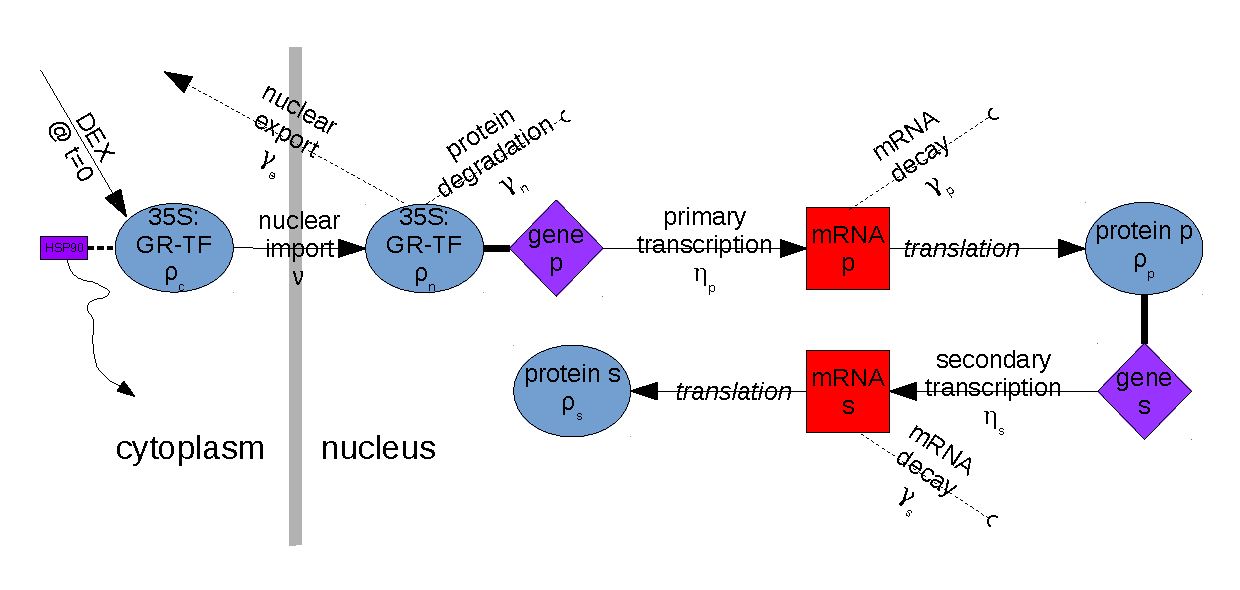
\includegraphics[width=\figwidth]{schematic}

  \subsection*{Nuclear import model}

  Transport of a glucocorticoid receptor (GR) into the nucleus after DEX application has been measured in animal tissue by several groups.

  \begin{minipage}[t]{1.0\linewidth}
    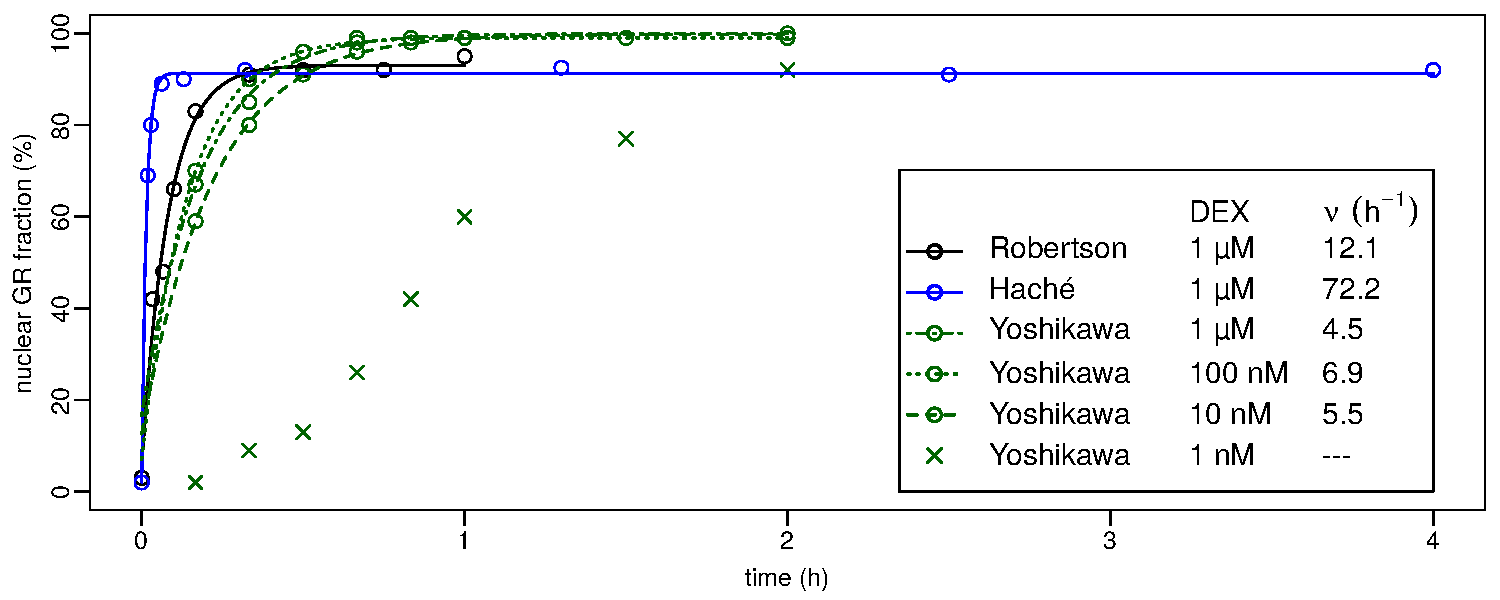
\includegraphics[width=\figwidth]{robertson-hache-yoshikawa}
    \captionof{figure}{
      The measured nuclear GR concentration follows a saturated exponential time course, except at very low DEX concentration. Data sources in References.
    }
  \end{minipage}
  
  The measured time courses are well described by a pair of linear ODEs:
  \begin{eqnarray*}
    \dot{\rho_c} &=& -\nu \rho_c + \gamma_e \rho_n \\
    \dot{\rho_n} &=&  \nu \rho_c - \gamma_e \rho_n - \gamma_n \rho_n
  \end{eqnarray*}
  \begin{eqnarray*}
    \rho_c &=& \text{\small cytoplasmic GR protein concentration} \\
    \rho_n &=& \text{\small nuclear GR protein concentration} \\
    \nu &=& \text{\small nuclear import rate} \\
    \gamma_e &=& \text{\small nuclear export rate} \\
    \gamma_n &=& \text{\small rate of loss of GR-TF from other causes}
  \end{eqnarray*}
  We neglect nuclear export and loss setting $\gamma_e=0$ and $\gamma_n=0$ since those rates are slow compared to our two-hour measurement span.
  We assume that import of chimeric GR-TF is similar to the published GR import data.

  \subsection*{Transcription model}

  We model altered transcription of target mRNA due to DEX-induced import of the GR-TF with a set of coupled ODEs:
  \begin{eqnarray*}
    \dot{\rho_p} &=& \eta_p \rho_n  - \gamma_p \rho_p  \\
    \dot{\rho_s} &=& \eta_s \rho_p  - \gamma_s \rho_s
  \end{eqnarray*}
  \begin{eqnarray*}
    \rho_p &=& \text{\small expressed mRNA/protein of a primary target of the GR-TF} \\
    \rho_s &=& \text{\small expressed mRNA/protein of a secondary target of the GR-TF} \\
    \gamma_p &=& \text{\small loss rate of primary mRNA/protein} \\
    \gamma_s &=& \text{\small loss rate of secondary mRNA/protein} \\
    \eta_p &=& \text{\small transcription rate between the GR-TF and primary target} \\
    \eta_s &=& \text{\small transcription rate between the primary and secondary targets}
  \end{eqnarray*}
  We assume that mRNA and protein concentrations are in fixed proportion, so that $\rho_p$ and $\rho_s$ represent measured mRNA levels as well as protein concentration.
  (This avoids two more equations and four more fit parameters accounting for translation.)
  $\gamma_p$ and  $\gamma_s$ represent loss of mRNA.
  
  These equations can be solved analytically; we set $\nu=10 {\rm h}^{-1}$ based on the animal tissue studies (\textit{we need to measure it!}).
  
  \subsection*{Primary target expression time course metrics}
  
  \textbf{The model provides two independent time course metrics:}
  \begin{itemize}
  \item $\hat{\eta}_p  \equiv \eta_p \rho_n(0) / \rho_p(0)$ characterizes the \textit{initial change} of mRNA level.
  \item $\gamma_p$ characterizes the \textit{loss} of mRNA.
  \end{itemize}
  In addition, we derive an asymptotic $t$$\rightarrow$$\infty$ fold change:
  \begin{equation*}
    {\rm logFC}_\infty \equiv \lim_{t \to \infty} \log_2\frac{\rho_p(t)}{\rho_p(0)} = \log_2\left(1 + \frac{\hat{\eta}_p}{\gamma_p} \frac{\rho_c(0)}{\rho_n(0)} \right)
  \end{equation*}
  The ratio $\hat{\eta_p}/\gamma_p$ therefore determines the asymptotic fold change of a transcript: \textbf{mRNA transcription and loss play equal roles in the final transcript level}.

  \subsection*{Time-course DEX-induced GR-TF expression measurements in {\it Arabidopsis thaliana}}
  
  The WT and five GR-TF Col-0 plant lines were grown to seedlings, and tissue was exposed to 50 $\mu$M of DEX and flash frozen 0, 0.5, 1 and 2 hours later.
  Almost all GR-TF samples had three biological replicates per time (WT had six). RNA was extracted and assayed with the Affymetrix ATH1 microarray and Illumina HiSeq RNA-seq.
  The microarray data were analyzed using the R packages \texttt{affy} and \texttt{limma}; the RNA-seq data were analyzed using TopHat2, Cufflinks and Cuffdiff.
  Sequences were mapped to the TAIR10 reference genome.

  %----------------------------------------------------------------------------------------
  %	RESULTS 
  %----------------------------------------------------------------------------------------

  \section*{RESULTS}

  
  \subsection*{Time courses exhibit qualitative variation}

  \textbf{\underline{When} you measure DE in an induced expression experiment is important!}
  
  \begin{minipage}[t]{1.0\linewidth}
    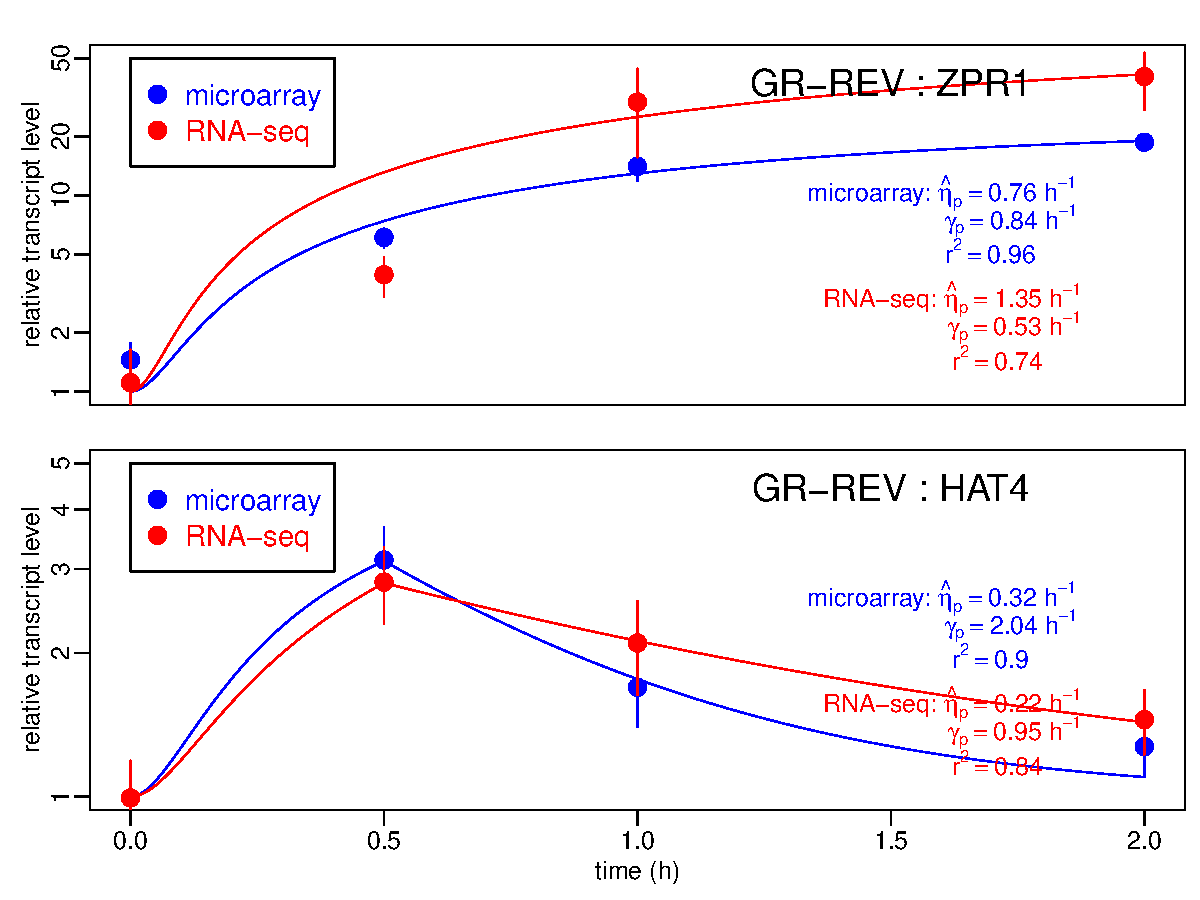
\includegraphics[width=\figwidth]{ZPR1-HAT4}
    \captionof{figure}{
      Expression time courses vary greatly, from strong GR-REV monotonic risers like \textit{ZPR1} to HD-ZIPII self-regulators like \textit{HAT4}. Lines represent primary target model fits
      with transcription turned off at t=30 mins for \textit{HAT4}. (\textit{HAT4} turn-off occurs some time between t=15 and 45 mins.)
    }
  \end{minipage}

  \subsection*{Model parameters $\hat{\eta}_p$ and $\gamma_p$ distinguish time course shapes}

  \textbf{The induced expression change can be large due to high transcription rate and/or low transcript loss.}
  Asymptotic fold change differs greatly from that measured at individual times after DEX application.
  
  \begin{minipage}[t]{1.0\linewidth}
    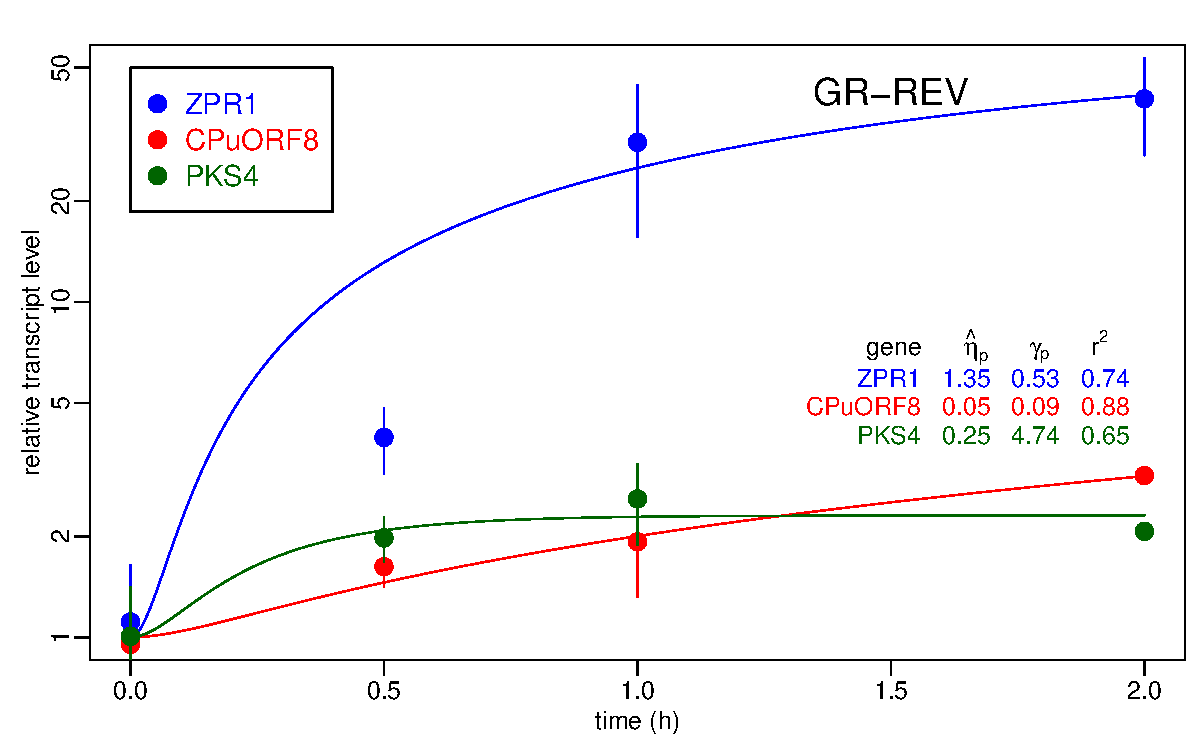
\includegraphics[width=\figwidth]{ZPR1-CPuORF8-PKS4}
    \captionof{figure}{
      Distinct time course shapes result from different transcription strength vs.\ loss rate for these GR-REV targets:
      high $\hat{\eta}_p$, low $\gamma_p$ for \textit{ZPR1}, the most strongly regulated GR-REV target; 
      low $\hat{\eta}_p$, low $\gamma_p$ for \textit{CPuORF8}, which reaches a significant fold-change due to low loss;
      and high $\hat{\eta}_p$, high $\gamma_p$ for \textit{PKS4}, which saturates quickly due to high loss. (RNA-seq data.)
    }
  \end{minipage}

  \subsection*{Down-regulated transcripts are also well fit}

  \begin{minipage}[t]{1.0\linewidth}
    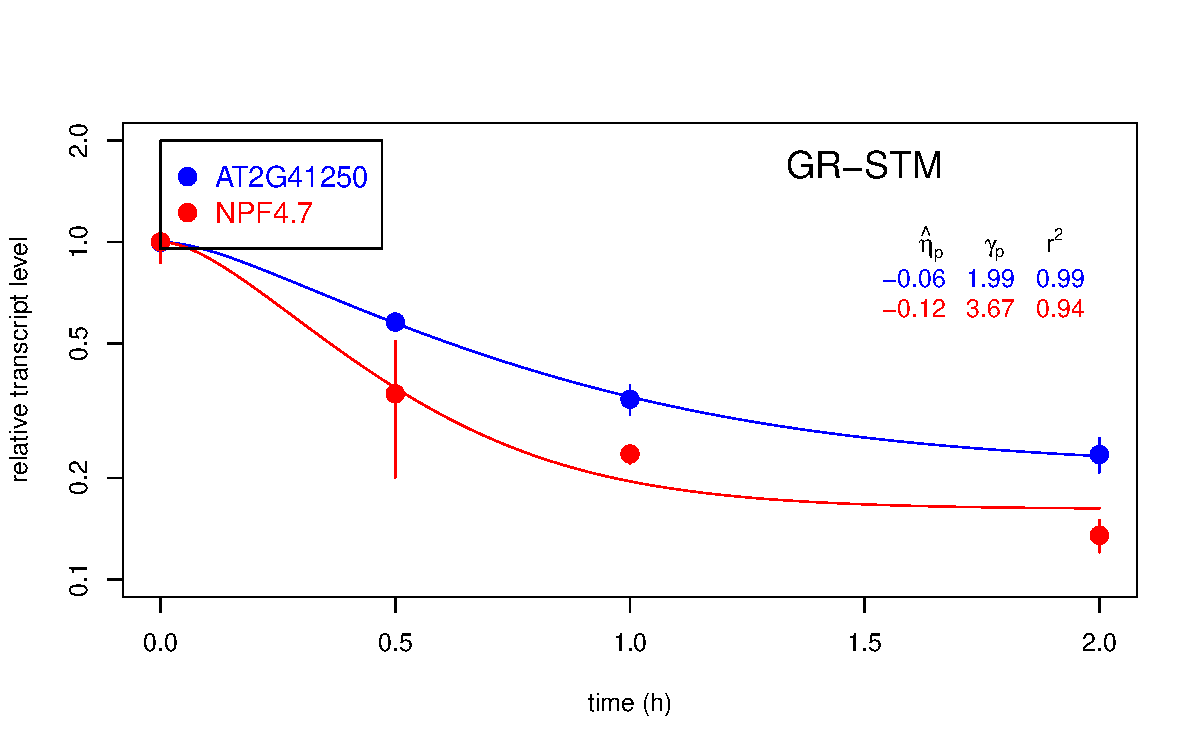
\includegraphics[width=\figwidth]{At2g41250-NPF47}
    \captionof{figure}{
      \textit{GR-STM} has many down-regulated targets; these two are particularly well fit by the model. (RNA-seq data.)
    }
  \end{minipage}
  
  \subsection*{Example: A down-regulated target of \textit{HAT22}?}

  \begin{minipage}[t]{1.0\linewidth}
    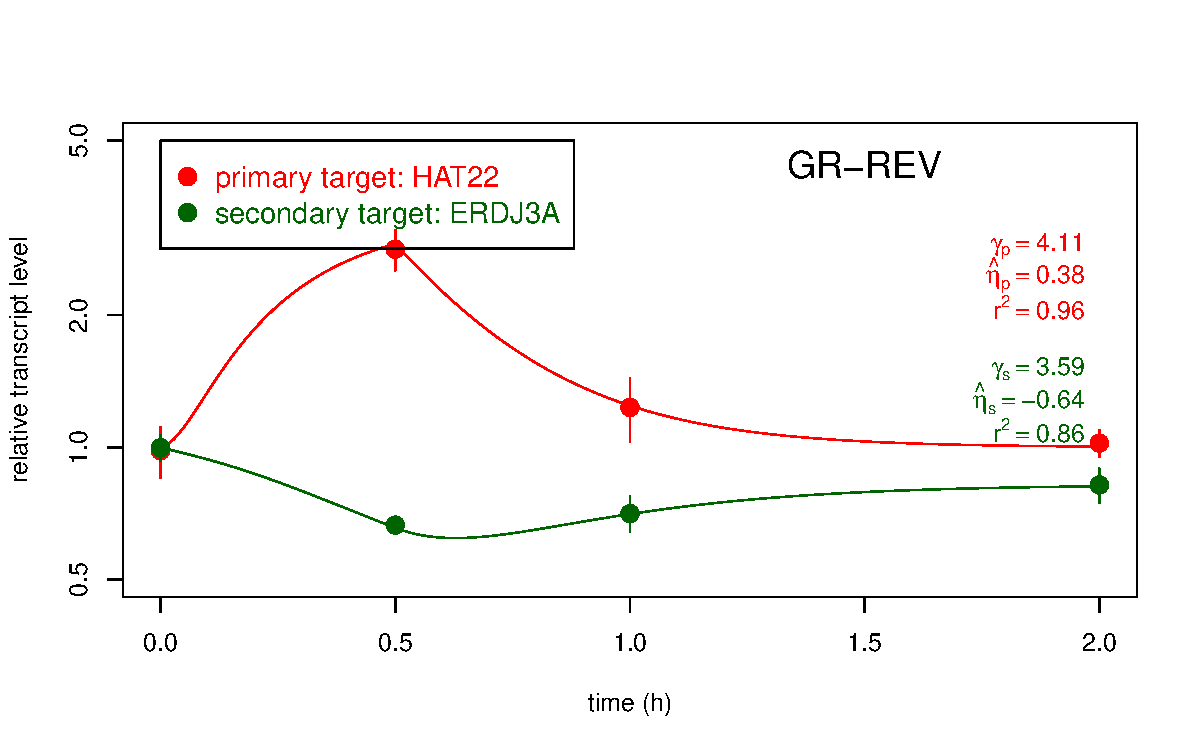
\includegraphics[width=\figwidth]{HAT22-ERDJ3A}
    \captionof{figure}{
      \textit{HAT22} is a self-regulating target of \textit{REV} which is also a TF. \textit{ERDJ3A} may be a \textit{down}-regulated target of \textit{HAT22} which returns
      to its WT level after \textit{HAT22} turns off. (Microarray data.)
    }
  \end{minipage}

  
  %----------------------------------------------------------------------------------------
  %	CONCLUSIONS
  %----------------------------------------------------------------------------------------

  \section*{CONCLUSIONS}
  \color{CarnegiePriBlue}
  
  \begin{enumerate}
  \item DEX-induced expression of GR-TF targets exhibits a variety of time courses, requiring better quantification than single-time fold change.
  \item Time courses can be fit by a basic ODE model with three shape parameters describing transcription strength, transcript loss and, when needed, turn-off.
  \item The model simulates primary and secondary transcriptional responses, supporting target discovery and inference of gene regulatory networks.
  \end{enumerate}

  %----------------------------------------------------------------------------------------
  %	FURTHER RESEARCH
  %----------------------------------------------------------------------------------------

  \section*{Further Research}
  
  \begin{enumerate}
  \item Improve model to make robust fits for ``black box'' analysis, perhaps in a Web application
  \item Study tighter time course of selected GR-TFs and targets using both RNA-seq and qPCR
  \item Measure GR-TF nuclear import using flourescent probes or other technique
  \item Measure mRNA induction in real time with CRISPRi activation?
  \end{enumerate}

  %----------------------------------------------------------------------------------------
  %	REFERENCES
  %----------------------------------------------------------------------------------------

  \nocite{*} % Print all references regardless of whether they were cited in the poster or not
  \bibliographystyle{plain} % Plain referencing style
  \bibliography{hokin-aspb2017} % Use hokin-aspb2017.bbl - regenerate with bibtex

  %----------------------------------------------------------------------------------------
  %	ACKNOWLEDGEMENTS
  %----------------------------------------------------------------------------------------

  {\small This research was funded by National Science Foundation grant \#0929413.}
  
  
\end{multicols}
\end{document}
